\chapter{Continuous Random Variables}
\begin{stbox}{General Information}
  \begin{itemize}
    \item A function \(f \colon \mathbb{R}\to \mathbb{R}\) is a \emph{probability density function} (pdf) of a continuous random variable \(X\) iff \(f\) is nonnegative and \(\int_{-\infty}^{\infty}f(x)\,dx=1\).
    \item For any probability mass function \(f\), we have \(\Prob(a\leq X\leq b)=\int_{a}^{b}f(x)\,dx\). Whether the inequality is strict or nonstrict does not affect the above identity. 
    \item A \emph{mode} of \(X\) is any value \(m\) such that \(f(m)\) is maximum.
    \item A \emph{cumulative distribution function} (cdf) \(F \colon \mathbb{R}\to [0,1]\) of a random variable \(X\) is defined by
    \[F(x)\coloneq P(X\leq x)=\int_{-\infty}^{x}f(x)\,dx.\]
    \item When writing out the cdf as a piecewise function, we explicitly write out the range of values for each case. We reserve the use of ``otherwise'' for pdf's.
    \item Any cdf is continuous and nondecreasing.
    \item Let \(X\) be a continuous random variable with cdf \(F\). To find the pdf \(g\) of any \(Y(X)\), we first find its cdf, then differentiate. We achieve this by reverse engineering \(Y(X)\leq y\) to find an inequality that relates \(X\) with \(y\). E.g. \(e^X\leq y\) iff \(X\leq \ln(y)\).
  \end{itemize}
\end{stbox}
\begin{note}
  It is important to check whether \(Y(X)\) is an increasing or decreasing function.
\end{note}
\begin{example}{An increasing \(Y(X)\).}{}
  Let \(Y=e^X\). Then,
  \[\Prob(Y\leq y)=\Prob(e^X\leq y)=\Prob(X\leq\ln(y)).\]
\end{example}
\begin{example}{A decreasing \(Y(X)\).}{}
  Let \(Y=e^{-X}\). Then,
  \[\Prob(Y\leq y)=\Prob(e^X\leq y)=\Prob(X\geq\ln(y)).\]
\end{example}
\begin{example}{Another decreasing \(Y(X)\).}
  Let \(X\sim\operatorname{U}(0,\pi/2)\) and \(Y=\cos(X)\). Then, 
  \[\Prob(Y\leq y)=\Prob(\cos(X)\leq y)=\textcolor{green!70!black}{\Prob(X\leq\pi/2-\cos^{-1}(y))}\neq \textcolor{red}{\Prob(X\leq\cos^{-1}(y))}.\]
  \begin{figure}[H]
    \centering
    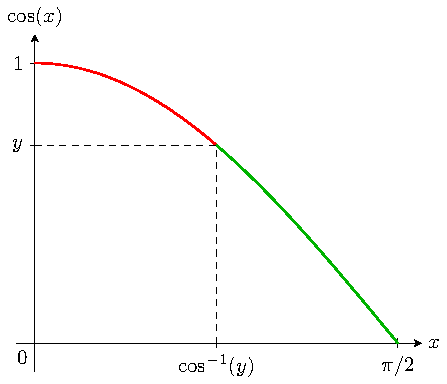
\includegraphics{Diagrams/CRV-cosine/diagram.pdf}
    \caption{The graph of \(\cos(x)\) against \(x\). Notice that \textcolor{green!70!black}{\([\cos^{-1}(y),\pi/2]\stackrel{\cos}{\to}[0,y]\)}, while \textcolor{red}{\([0,\cos^{-1}(y)]\stackrel{\cos}{\to}[y,1]\)}.}
    \label{fig:CRV-cosine}
  \end{figure}
\end{example}
\begin{stbox}{}
  \begin{itemize}
    \item A \emph{median} of \(X\) is any value \(m\) such that \(\Prob(X\leq m)=F(m)=1/2\).
    \item Mean/Expectation: 
    \[\mu=\E(X)\coloneq \int_{-\infty}^{\infty}xf(x)\,dx \qquad\text{and}\qquad \E(g(X))=\int_{-\infty}^{\infty}g(x)f(x)\,dx.\]
    \item Important property: 
    \[\E(ag(X)\pm bh(x))=a\E(g(X))\pm\E(h(X)).\]
    \item Variance: 
    \[\Var(X)\coloneq \E(X^2)-[\E(X)]^2.\]
    \item Important property:
    \[\Var(aX\pm b)=a^2\Var(X).\]
  \end{itemize}
\end{stbox}